\chapter{Revisão da literatura}

\section{Contextualização Teórica}
Esta seção apresenta alguns dos termos comumente utilizados na gestão de receitas no transporte ferroviário de passageiros, além de aprofundar-se em conceitos específicos que frequentemente geram confusão entre si.

\begin{description}[style=unboxed, leftmargin=0cm]

	\item[Viagem:] Um trem programado para uma data específica é denominado "viagem". Uma viagem inclui uma estação de partida (estação de origem) e uma estação de chegada (estação de destino final). Exemplo: O trem \#03450-1 de 12 de janeiro de 2024 é uma viagem:

        \begin{figure}[H]
            \begin{center}
                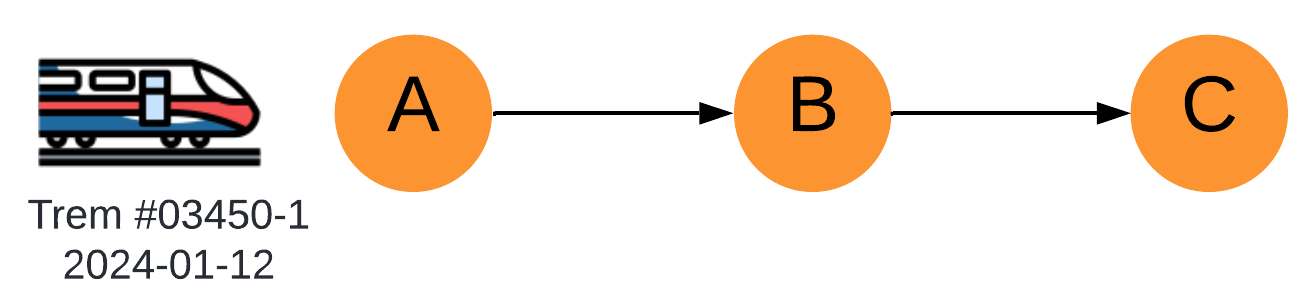
\includegraphics[scale=0.12]{img/viagem.png}
                \label{fig: viagem}
            \end{center}
        \end{figure}
         \vspace{-1cm}

	\item[Trecho e itinerário:] Um trecho é uma conexão direta entre duas estações.

        \begin{figure}[H]
            \begin{center}
                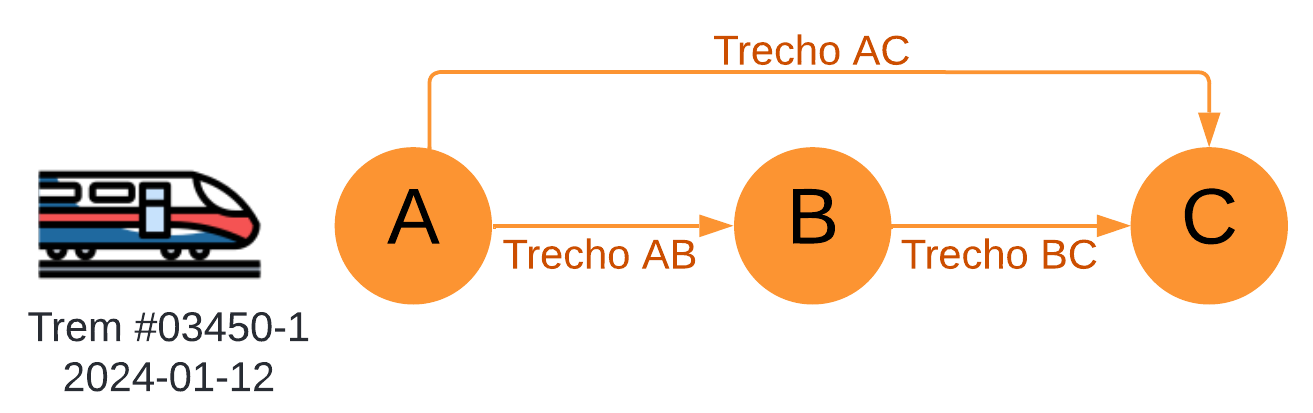
\includegraphics[scale=0.12]{img/trecho.png}
                \label{fig: trecho}
            \end{center}
        \end{figure}

    Um itinerário é uma combinação única de origem, destino, horário de partida e trem. Um itinerário pode consistir em um ou mais trechos, e uma viagem pode englobar um ou mais itinerários.

        \begin{figure}[H]
            \begin{center}
                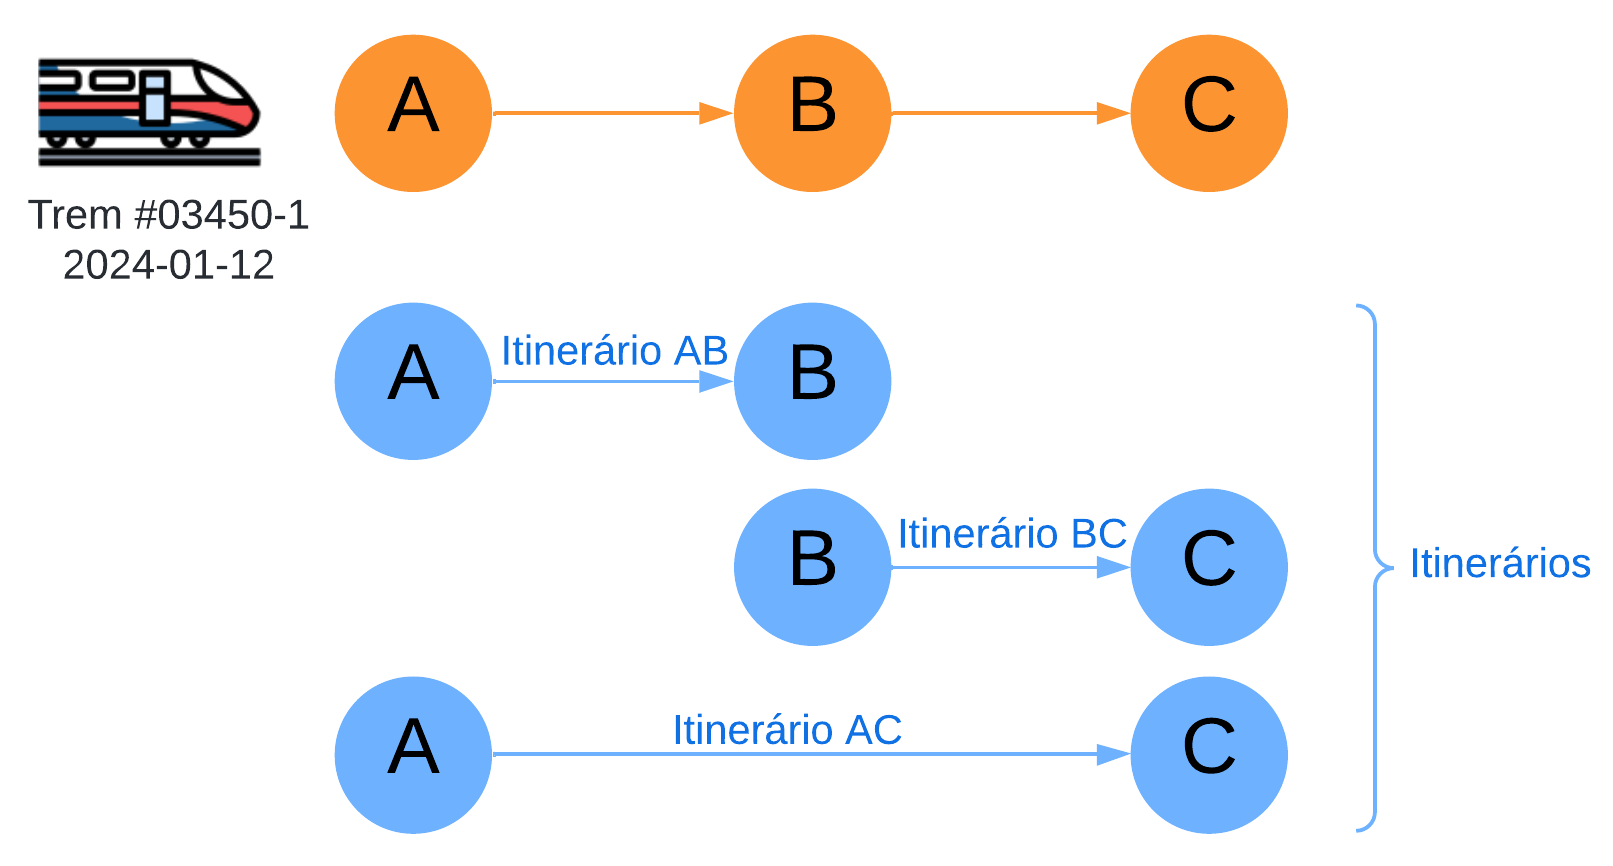
\includegraphics[scale=0.12]{img/itinerario.png}
                \label{fig: itinerario}
            \end{center}
        \end{figure}
        \vspace{-1cm}

	\item[Classes de controle:] Uma classe de controle é um produto oferecido por um operador de transporte a passageiros potenciais por um preço específico. As classes de controle também são conhecidas como classes tarifárias, produtos tarifários ou classes de reservas. Uma classe de controle define os benefícios e/ou restrições que o passageiro terá como resultado do preço pago pelo bilhete.

	\item[Horizonte de reserva:] É o período de tempo entre o momento em que os bilhetes para o trem em questão são disponibilizados para venda pela primeira vez e a data de partida do trem. O horizonte de reserva geralmente é discretizado por dias, de forma que cada período representa um dia específico antes da partida (DBD). Frequentemente, realizamos uma agregação temporal para reduzir o tamanho do horizonte de reserva, selecionando alguns DBD específicos como pontos de controle (CP). Nesse contexto, o horizonte de contabilização é discretizado por períodos, onde o tamanho de cada período corresponde ao intervalo de tempo entre dois CP consecutivos.

        \begin{figure}[H]
            \begin{center}
                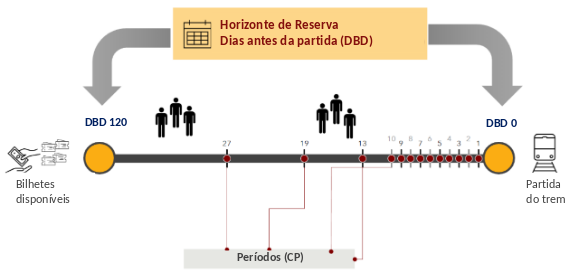
\includegraphics[scale=0.53]{img/h_reserva.png}
                \caption{Horizonte de reserva}
                \label{fig: h_reserva}
            \end{center}
        \end{figure}

	\item[Reservas:] As reservas representam o número de assentos protegidos para atender à demanda potencial de uma classe de controle específica em um determinado itinerário, durante um período específico do horizonte de reserva. O tamanho da reserva é definido no processo de otimização, considerando a demanda potencial do itinerário e da classe de controle correspondente. As reservas também são conhecidas como níveis de proteção.

	\item[Autorizações:] As autorizações representam o número de assentos disponíveis para venda em um determinado itinerário e classe de controle. Elas podem ser entendidas como a quantidade de bilhetes apresentados aos passageiros como disponíveis para compra. As autorizações têm como objetivo controlar o volume de passageiros ao longo de um itinerário ou trecho.

	\item[Demanda comportamental:] Neste modelo, assume-se que o comportamento de compra dos passageiros é influenciado pelo conjunto de classes de controle disponíveis. Um exemplo desse conceito é ilustrado na Figura \ref{fig: dc1}. Considere um cenário em que 4 clientes desejam comprar a tarifa A3, sendo essa sua primeira opção. Caso a tarifa A3 não esteja disponível, um dos clientes desiste da compra, enquanto os outros 3 permanecem no sistema e estão dispostos a adquirir a tarifa A2. Se A2 também não estiver disponível, mais 2 clientes abandonam a compra, restando apenas um cliente que opta por A1 (geralmente, a opção de maior valor).

        \begin{figure}[H]
            \begin{center}
                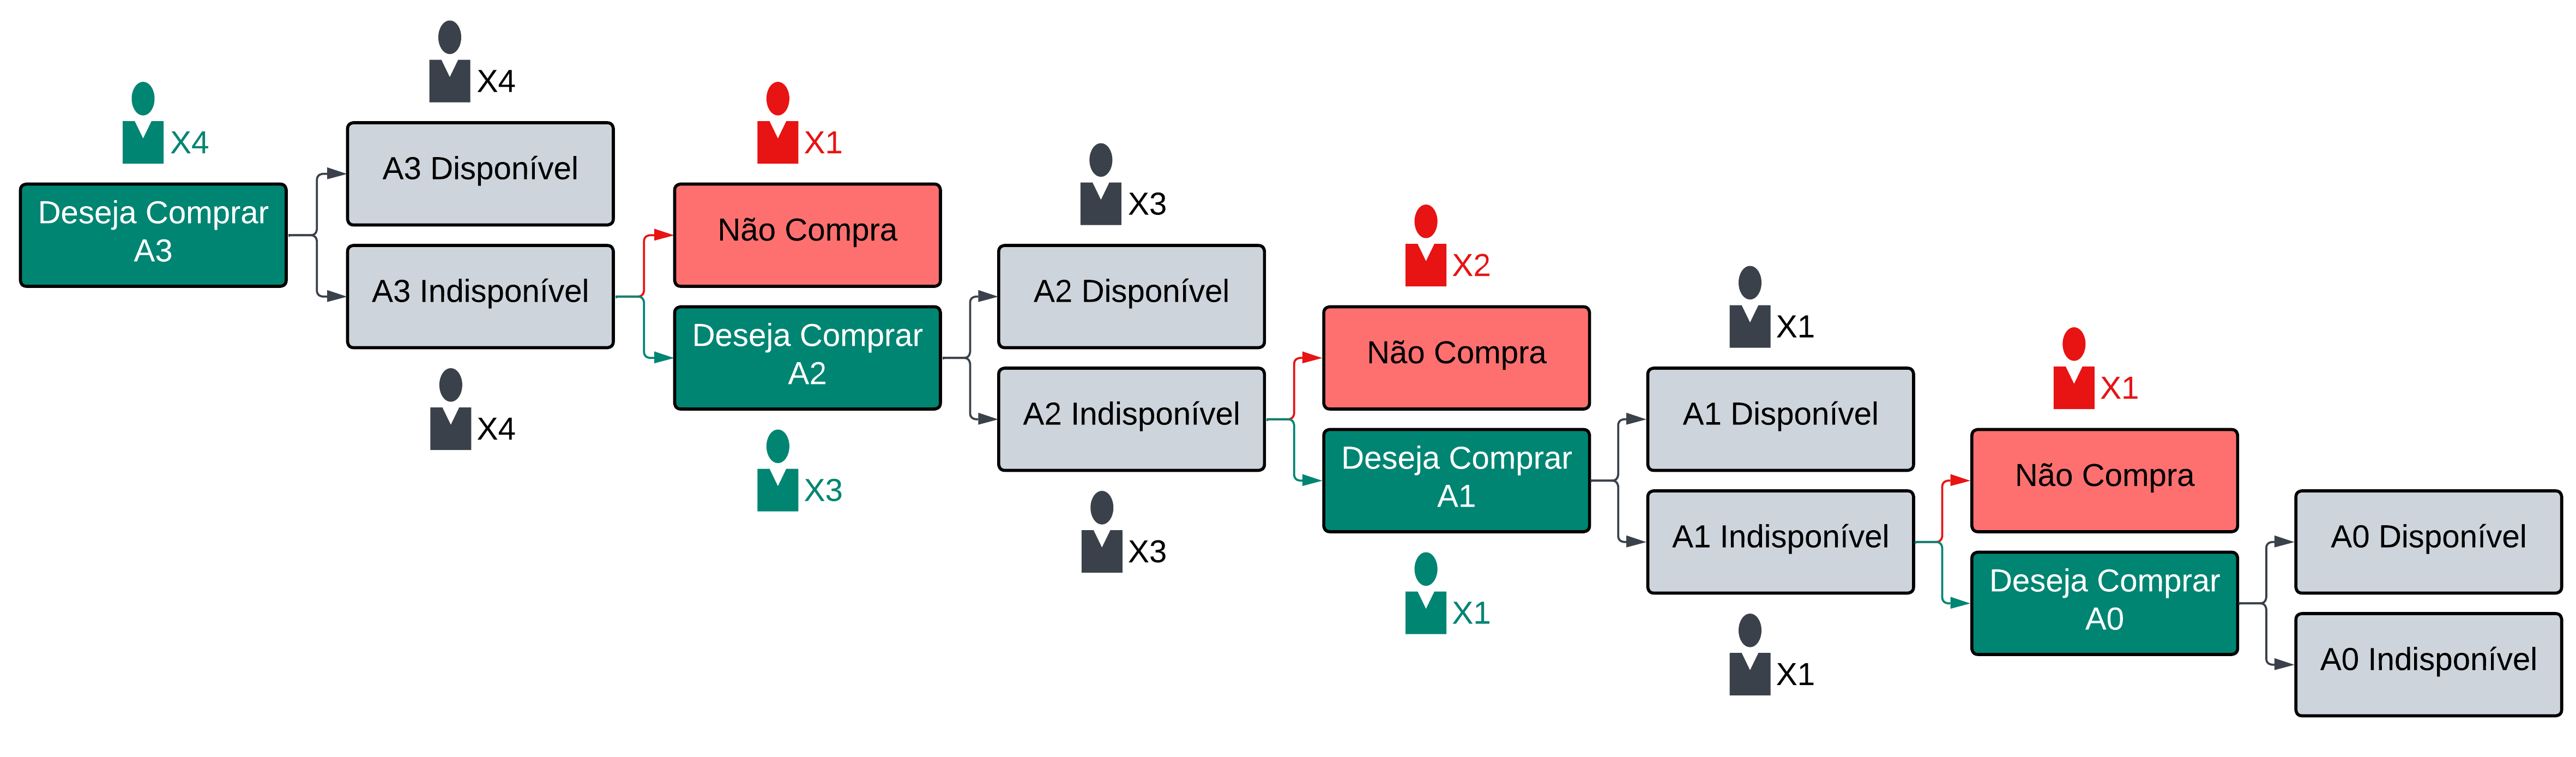
\includegraphics[scale=0.09]{img/dc1.png}
                \caption{Representação de demanda comportamental}
                \label{fig: dc1}
            \end{center}
        \end{figure}

    \item[Demanda independente:] Os clientes compram um produto específico, independentemente da oferta disponível no momento. Em um modelo de demanda independente, assume-se que um cliente disposto a pagar R\$100 por um bilhete nunca optaria por um bilhete mais barato (por exemplo, R\$50), mesmo que este estivesse disponível.
    
        \begin{figure}[H]
            \begin{center}
                
\includegraphics[scale=0.7]{img/di1.png}
                % \caption{Representação de demanda independente}
                \label{fig: di1}
            \end{center}
        \end{figure}
        \vspace{-1cm}
        
    \item[Skip lagging:] No contexto do transporte ferroviário de passageiros, skip lagging refere-se a uma estratégia de otimização na programação das paradas dos trens, na qual certos serviços omitem paradas intermediárias em determinados trechos. O objetivo é reduzir os tempos de viagem e aumentar a eficiência operacional, garantindo que essa omissão não comprometa a acessibilidade e a qualidade do serviço oferecido aos passageiros. Na seção de modelagem matemática, será apresentado um conjunto de restrições associadas a esse conceito.
    
    \item[Fulfillments over periods:] No contexto do transporte ferroviário de passageiros, fulfillments over periods refere-se ao cumprimento de determinados níveis de serviço, demanda ou capacidade ao longo de um período de tempo definido. Esse conceito é especialmente relevante na gestão de receitas, planejamento operacional e alocação de recursos, onde é essencial garantir que a oferta de serviços ferroviários atenda a objetivos estratégicos ao longo do tempo, em vez de se concentrar apenas em momentos específicos. Na seção de modelagem matemática, será apresentado um conjunto de restrições associadas a esse conceito.
\end{description}


\section{Revenue Management (RM)}
A gestão da receita, conhecido como RM, do inglês \textit{Revenue Management}, desempenha um papel essencial na otimização da rentabilidade das empresas, permitindo ajustes dinâmicos nos preços e na capacidade de oferta conforme a demanda em tempo real \parencite{Gallego1994}. Essa abordagem estratégica é particularmente relevante em setores onde os recursos são limitados, como na aviação, hotelaria e transporte ferroviário. Nessas indústrias, cada unidade de capacidade disponível precisa ser aproveitada ao máximo, e o RM possibilita exatamente isso, segmentando clientes, controlando a disponibilidade de produtos e ajustando preços de forma dinâmica \parencite{HEO2009446}. Além de elevar a rentabilidade, essa estratégia melhora a previsibilidade da demanda, permitindo que as empresas reajam rapidamente às oscilações do mercado. Em um ambiente altamente competitivo, o gerenciamento de receitas torna-se um diferencial crucial para manter uma posição sólida e, ao mesmo tempo, oferecer soluções mais eficientes e personalizadas para os consumidores.

Até o ano de 1978, a Junta de Aeronáutica Civil (CAB em inglês) limitava a concorrência entre as companhias aéreas, onde basicamente as companhias só podiam competir oferecendo serviços como refeições luxuosas e alta frequência nos horários de saída dos voos. Nesse ponto, a CAB não permitia que fosse oferecida uma tarifa menor para um voo, se esta fosse antieconômica para a indústria como um todo. Assim, mesmo que para uma companhia aérea fosse rentável colocar um valor baixo para uma passagem em comparação com outra, a CAB não permitiria, a menos que houvesse uma justificativa extremamente sólida. Quando esse tipo de situação ocorria, o restante das companhias aéreas justificava que o público seria prejudicado, pois elas teriam que aumentar o valor das passagens em outras rotas para compensar o baixo custo da nova proposta do concorrente \parencite{article_base}.

Com a chegada da desregulamentação, as companhias aéreas se depararam com um mundo cheio de novas formas de concorrência, onde o preço das passagens se tornou prioritário. E foi nesse momento que iniciou a verdadeira concorrência entre as transportadoras. Aqui surgiu um novo problema em função da diversidade de preços com diferentes restrições que limitam a disponibilidade de assentos a tarifas mais baixas, a presença de múltiplos voos operados por diversas companhias aéreas em diferentes rotas, e a variabilidade na demanda por assentos em função de fatores como a temporada, o dia da semana, a hora do dia e a qualidade do serviço oferecido, o que influencia a escolha dos passageiros entre diferentes opções de voo \parencite{article_base}.

Nesse momento, esse problema foi denominado como problema de preços e combinação de passageiros e foi modelado como: cada passageiro em um voo representa um custo de oportunidade, já que sua ocupação de um assento impede que outro passageiro com um itinerário mais rentável ou uma classe de tarifa mais alta o utilize. Isso se traduz na possibilidade de assentos vazios em diferentes segmentos de voo, o que afeta a eficiência da rede da companhia aérea ao considerar múltiplos passageiros com diversas origens, destinos e classes de tarifas \parencite{article_base}.

Houve dois possíveis resultados: 1) a otimização da combinação de passageiros permite que as companhias aéreas estruturem de maneira mais eficaz seu sistema de reservas, estabelecendo limites e prioridades adequadas para o número de passageiros com diferentes classes de tarifas em distintos voos. 2) Além disso, possibilita a avaliação de diversos cenários de preço e rota, considerando o benefício gerado a partir da melhor combinação de passageiros em relação a um cenário específico.

Ao ajustar a estrutura das classes de tarifas, as companhias aéreas buscam gerenciar o deslocamento de passageiros por meio de estratégias de preços e a aplicação de restrições como horários, duração da estadia e tempo de antecedência à saída do voo. Além disso, buscam reduzir o deslocamento controlando a capacidade, determinando a quantidade de assentos atribuídos a cada classe de tarifa em cada segmento de voo.

Por outro lado, a otimização da combinação de passageiros é formulada como: "Dada a previsão diária da demanda de passageiros nas diferentes classes de tarifas, qual combinação de passageiros e classes de tarifas em cada segmento de voo maximizará as receitas do dia?" Essa resposta ajuda a companhia aérea a determinar a alocação ideal de reservas entre as diversas classes de tarifas em cada segmento de voo \parencite{article_base}.

Essas últimas duas definições foram conhecidas como Yield Management e, posteriormente, com a chegada de novos sistemas de informação, regras de controle e outras condições, foram generalizadas e aplicadas em outras indústrias de características semelhantes, que no futuro seriam chamadas de Revenue Management \cite{article_YM_to_RM}.

Según \cite{article_Ryzin2014}, a gestão de receitas (RM) abrange o conjunto de estratégias e táticas que as empresas utilizam para gerenciar de forma científica a demanda por seus produtos e serviços. Além disso, pode-se dizer que, seu objetivo é vender cada unidade de ações para o cliente certo, no momento e pelo preço corretos \cite{doi:10.1080/02642069.2010.491543}.

A princípio, os problemas de gestão de RM parecem ser simples; no entanto, nada poderia estar mais longe da realidade. Esses problemas têm uma complexidade esmagadora, e este documento não seria suficiente para detalhar cada um deles, apenas para mencionar alguns, temos modelagem, análise teórica, implementação, previsão, vendas excessivas, controle de estoque de assentos, preços, etc. Então, como sempre acontece, trabalha-se com simplificações de fatores muito complexos e com aproximações em outros casos \cite{doi:10.1287/trsc.33.2.233}.


\subsection{Modelagem do Transporte Ferroviário de Passageiros}
Nos últimos anos, a gestão de reservas de bilhetes no transporte ferroviário de passageiros evoluiu significativamente graças à aplicação de modelos matemáticos avançados. Esses modelos têm como objetivo otimizar a alocação de assentos, o planejamento de paradas e as estratégias de preços, buscando maximizar as receitas e melhorar a satisfação dos passageiros. A seguir, são descritos alguns dos enfoques mais relevantes utilizados nesse campo, com base em pesquisas recentes.

Um dos modelos destacados é o desenvolvido por \cite{zhou2023pricing}, que integra a teoria das perspectivas, o modelo logit e um modelo de transferência de fluxo de passageiros para alocar a demanda de maneira eficaz. Esse enfoque permite estabelecer preços diferenciados e distribuir os assentos de forma a maximizar as receitas, considerando as preferências e comportamentos de diferentes segmentos de passageiros.

Por outro lado, o planejamento das paradas dos trens e a estratégia de preços estão interligados e impactam tanto as receitas quanto a experiência dos passageiros. Em \cite{zhou2022nonlinear} propuseram um modelo de otimização não linear inteiro misto que aborda conjuntamente a estratégia de preços dos bilhetes e o planejamento das paradas. Esse modelo busca maximizar as receitas do transporte ferroviário e minimizar o tempo de viagem dos passageiros, alcançando um equilíbrio eficiente entre oferta e demanda.

Além disso, a demanda de passageiros está sujeita a incertezas que tornam a gestão operacional mais desafiadora. Han e Ren em 2020 desenvolveram um modelo que otimiza conjuntamente o planejamento de paradas e a alocação de bilhetes, utilizando a teoria da incerteza. Esse modelo busca maximizar a satisfação dos passageiros e a taxa média de ocupação dos assentos, oferecendo soluções robustas frente às flutuações na demanda \cite{han2020uncertainty}.

Posteriormente, em \cite{schoebel2021tariff}, investiga-se como a escolha da rota dos passageiros é influenciada pelas estruturas tarifárias e pelos preços dos bilhetes. Sua pesquisa abordou o problema de determinar a tarifa mais econômica em sistemas de transporte público, avaliando diferentes estruturas tarifárias, como aquelas baseadas em distância ou zonas, e propondo algoritmos altamente eficientes para resolver esses problemas.